\documentclass[11pt,a4paper]{article}

\usepackage[utf8]{inputenc}
\usepackage[T1]{fontenc}
\usepackage{amsmath,amssymb,amsthm}
\usepackage{graphicx}
\usepackage{booktabs}
\usepackage{hyperref}
\usepackage[margin=1in]{geometry}
\usepackage{natbib}
\usepackage{algorithm}
\usepackage{algpseudocode}
\usepackage{multirow}
\usepackage{xcolor}

\title{Topology Under-Determines Governance Maturity in Data Lineage\\
Graphs: A Negative Result and a Reusable Inference Protocol}

\author{
  Dineshkumar Malempati Hari \\
  \textit{University of the Cumberlands, Williamsburg, KY, USA} \\
  \texttt{mhdk.dinesh@gmail.com} \\
  \href{https://orcid.org/0009-0003-1036-9477}{orcid.org/0009-0003-1036-9477}
}

\date{July 2026}

\begin{document}
\maketitle

\begin{abstract}
Institutional theory holds that organizations under shared governance
pressures converge structurally. Carried over to the artifacts that
governance produces, the claim implies that better-governed data estates
should yield topologically distinct lineage graphs. The implication is
plausible and it follows from well-established theory, but we could find
no study that has tested it. We test it here. On a curated-metadata
production dbt estate with 18 analyzable domains, a spectral descriptor
correlates strongly with documentation rate (Spearman $\rho = -0.71$,
bootstrap 95\% CI $[-0.92, -0.27]$). The correlation is not what it
looks like. Algebraic connectivity takes exactly three values across the
eighteen domains, one per architectural layer, and it is constant inside
every layer. Twelve source-only domains carry no internal edges, so
$\lambda_2 = 0$. Five staging domains are stars, and a star with more
than one leaf has algebraic connectivity of exactly 1. The single mart
sits between the two at $0.168$. A layer-stratified
permutation test consequently returns $p = 1.000$, because every
admissible relabelling reproduces the observed correlation exactly. The
association orders three architectural layers and does nothing else. A
rank-degeneracy power analysis puts the observed
effect at the design's minimum detectable size. The relationship does
not replicate on two public dbt projects, though the non-replication is
confounded with a domain-construct mismatch we make explicit. A
persistent-homology descriptor reduces exactly to the cycle-rank
baseline ($\rho = +1.000$) on real graphs, and a node-importance
prediction (AUC 0.90) reproduces a published centrality finding rather
than extending it. We offer two things. The first is a bounded negative
result. Lineage topology is a poor proxy for governance maturity once
the architectural-layer confound is removed, and that confound is no
accident of this estate but a consequence of how layered analytics
estates are built, so more data of the same kind will not repair it. The
second is an inference protocol for small-$n$ graph-descriptor
correlation studies. We borrowed most of it, restricted permutation from
experimental design and degree-preserving rewiring from network science,
composed the way network neuroscience composes its null models. The
rank-degeneracy diagnostic is the part we have not found elsewhere. It
counts distinct descriptor values within each stratum and flags a
degenerate design before anyone believes the correlation.
\end{abstract}

\smallskip
\noindent\textbf{Keywords:} data governance, lineage graphs, community detection, spectral graph theory, persistent homology, structural descriptors, network analysis

\section{Introduction}

Data governance frameworks specify how organizations should manage data
assets. They set out who owns an asset, how its quality is assured, what
documentation exists, and how changes propagate through transformation
pipelines. Mature governance is supposed to show up as clear domain
boundaries, tested transformations, and documented interfaces between
pipeline stages. Immature governance shows up as orphaned assets,
unclear ownership, redundant paths, and untested transformations.

None of that is assessed structurally in practice. The dominant approach
is self-assessment against capability models such as DAMA-DMBOK
\citep{dama2017} or DCAM, which are reference guides rather than
maturity ladders, and which record stated policy rather than the
organization of the assets themselves. Commercial catalog and
observability tooling automates that idea without changing it, deriving
governance and trust scores from metadata completeness, policy and
glossary coverage, stewardship workflow, declared tests, ownership and
usage. We know of no product that derives a governance score from a
topological property of the lineage graph.

\subsection{Where the structural hypothesis comes from}

The structural hypothesis is a live one all the same, and its warrant is
theoretical. \citet{dimaggio1983} argue that coercive, mimetic and
normative pressures drive organizations under a shared regime toward
structural convergence, and \citet{scott2013} develops the same logic
through regulative, normative and cultural-cognitive pillars. If data
governance is an institutional arrangement in that sense, organizations
governed alike should build alike, and the resemblance ought to be
legible in the artifacts governance produces. Lineage graphs are the
obvious artifact to look at. They are machine-readable, they fall out of
the transformation code rather than being authored for assessment, and
they record the dependency structure that governance is meant to
discipline.

We could not find prior work that states the implication in a form a
topological measurement could refute, so we state it ourselves and test
it rather than assume it. Operationally, if domain boundaries are
enforced, community detection at the appropriate resolution should
recover stable modular partitions. If transformations are tested, the
blast radius of any single failure should be concentrated rather than
diffuse. If the pipeline architecture is clean, the spectral properties
of the graph should reflect the coupling. If redundant dependency paths
exist, a sign of organic growth without architectural oversight,
persistent homology should detect reconvergent structure in the
undirected skeleton. Four descriptors, D1 through D4, operationalize
those four readings. They are the instrument under test, not the
contribution.

\subsection{What we found, and why it cannot be fixed with more data}

The instrument returns a strong reading and the reading is spurious. We
state that up front, ahead of the evidence, because the mechanism is
more useful to a reader than the null it produces. On the one production
estate in our sample that carries curated domain metadata, the D3
spectral descriptor correlates with documentation rate at $\rho = -0.71$
with a bootstrap interval clear of zero. Algebraic connectivity across
those eighteen domains takes three values and no others. Twelve
source-only domains have no internal edges at all, which forces
$\lambda_2 = 0$. Five staging domains are stars, and a star with more
than one leaf has algebraic connectivity of exactly 1. The single mart
sits at $0.168$. Within each of the three architectural
layers the descriptor is constant, so a layer-stratified permutation of
the governance labels cannot move the statistic and the test returns
$p = 1.000$.

The correlation therefore orders three architectural layers while
wearing the notation of a graph metric. Anyone who runs this study again
needs one further fact about it. The degeneracy is not small-sample bad
luck; it is what the layered build pattern produces. Raw sources are
landed without internal dependencies, staging models sit one-to-one over
those sources and so fan out from a shared parent, and joins are
deferred to the mart. An estate built that way decomposes into edgeless
domains, star-shaped domains, and a handful of reticulated mart domains,
and on the first two classes graph theory pins $\lambda_2$ at $0$ and at
$1$ irrespective of anything the organization does. Sampling more
estates of the same architecture supplies more observations at those
same three values. It supplies no new ones.

\subsection{Contributions}

\begin{enumerate}
  \item \textbf{A bounded negative result with its mechanism named.}
        Lineage topology under-determines governance maturity on the
        cleanest real data we could obtain. The apparent D3--documentation
        association ($\rho = -0.71$, bootstrap 95\% CI $[-0.92, -0.27]$)
        is carried entirely by architectural layer. Layer-stratified
        permutation returns $p = 1.000$ and the per-stratum count of
        distinct descriptor values is 1 in all three strata. We also give
        the graph-theoretic reason the degeneracy arises. That reason is
        what separates this from a null reported without explanation, and
        it tells a reader when to expect the same trap elsewhere.

  \item \textbf{An inference protocol for small-$n$ graph-descriptor
        studies, most of it transferred rather than invented.} The
        protocol collects permutation-based inference,
        Benjamini--Hochberg FDR correction over explicit hypothesis
        families, rank-residualization partial correlations, bootstrap
        intervals, degree-preserving and layer-preserving nulls,
        layer-stratified permutation, Louvain seed-robustness, and
        leave-scale-out cross-validation. Section~\ref{sec:protocol}
        traces every component to the discipline it came from. Only the rank-degeneracy diagnostic
        appears to be new. It counts distinct descriptor values per
        stratum and estimates the minimum detectable $|\rho|$ under the
        observed tie structure instead of a continuous assumption.

  \item \textbf{Precise descriptor definitions and implementation},
        including LWCC handling for disconnected graphs, combinatorial
        (unnormalized) Laplacian for D3, GUDHI parameters for D4
        (\texttt{max\_dimension=2}, $\mathbb{F}_2$ coefficients), and
        cycle rank baseline. All computations are reproducible from the
        public Zenodo archive.

  \item \textbf{Cross-dataset structural characterization.} D1--D4
        computed on 32 graphs from four heterogeneous sources (WfCommons
        scientific workflows, DLG-DG-23 Huawei Cloud lineage, DW-Bench
        warehouse schemas, anonymized production dbt manifest).
        Principal component analysis places production data lineage
        graphs in a distinct descriptor region marked by high community
        stability and small spectral gaps. This part is descriptive, it
        reproduces, and it needs no governance metadata, which is
        precisely why it survives while the governance claim does not.

  \item \textbf{Negative cross-organisation pilot at graph level with
        methodological caveat.} D3/documentation does not replicate to
        two public dbt projects (Cal-ITP, Mattermost) under
        folder-derived domain partitioning. We discuss why folder-derived
        domains are not the same construct as metadata-assigned dbt
        domains.

  \item \textbf{A reproduction of a published centrality result at node
        granularity.} On the DLG-DG-23 dataset with expert-annotated
        core data assets (36 labels across 6 Huawei Cloud graphs from
        Table 5 of \citep{chen2024dlgdg}), node-level topological
        descriptors trained on five graphs predict core-asset status in
        the held-out sixth graph at mean LR AUC $= 0.898 \pm 0.098$
        (LOGO cross-validation), substantially above random ($0.546$)
        and out-degree-only ($0.576$) baselines. This reproduces the
        node-centrality finding of \citet{chen2023centrality} on the
        same corpus, where the top predictors are PageRank and out-degree.
Phase
        5 evaluates ordinary node-level centrality, reachability, degree,
        and clustering features; it does not evaluate incremental D1--D4
        information. We report it as a reproduction, not as a new
        governance result.
\end{enumerate}

\section{Related Work}

\subsection{Governance Measurement}

Data governance frameworks define structural and procedural mechanisms
for data management \citep{khatri2010,abraham2019}. Assessment typically
relies on maturity models. DAMA-DMBOK \citep{dama2017} organizes eleven
knowledge areas as a reference guide rather than a prescriptive maturity
ladder, and DCAM evaluates institutional readiness. \citet{weber2009}
argue that governance design is contingent on organizational strategy,
which implies that a single maturity scale is insufficient.

Every one of these instruments measures declared policy, process, and
metadata. So does the commercial tooling that has grown up beside them,
which computes governance health and trust scores from metadata
completeness, glossary and policy coverage, stewardship workflow,
declared tests, ownership and usage. We are aware of no framework and no
product that reads a governance score off a topological property of the
lineage graph. We want to be clear about what follows from that. The
hypothesis this paper tests is not a claim that the field has asserted
and that we are refuting. It is a claim that the field's theory implies
and that nobody appears to have checked.

Institutional theory supplies that implication. \citet{dimaggio1983}
describe three isomorphic pressures, coercive, mimetic and normative,
that push organizations under shared governance regimes toward
structural convergence, and \citet{scott2013} extends the account
through regulative, normative and cultural-cognitive pillars. Take the
view seriously and a prediction follows. If governance is an
institutional arrangement, it should leave detectable structural
signatures in the artifacts it governs, and the lineage graph is the
artifact where such a signature would be cheapest to read. The rest of
this paper tests that prediction.

\subsection{Graph Analysis of Data Pipelines}

\citet{hou2026} apply temporal convolutional and graph convolutional
networks to data lineage DAGs for fault classification (1,240 nodes,
5,870 edges), achieving 95.8\% accuracy. Their work uses lineage
structure as input to prediction but does not extract governance-relevant
patterns from that structure.

Knowledge graph quality metrics \citep{seo2022} define six structural
measures for knowledge graphs. \citet{merono2024} position knowledge
graphs as governance backbones for AI systems. Neither applies
multi-scale graph descriptors to lineage topology.

An unpublished phase 0 feasibility analysis by the author
\citep{hari2026fractal} asked whether box-covering fractal dimension
could characterize a governance signal in data lineage. It could not.
Box-covering needs a diameter of roughly 8 or more and a locally
connected lattice-like topology before its scaling estimates stabilize,
and enterprise governance graphs supply neither. Lineage DAGs run to a
diameter of 3--6, entity-relationship graphs to 2--4 over a bipartite
hub topology, and product hierarchies are trees on which box-covering
is trivial. We read that as the geometry of the domain rather than a
deficiency in the data, since a well-governed lineage is a shallow DAG
by design. The descriptors used here were chosen to fit that geometry,
and we make no fractal claim about governance graphs anywhere in this
paper. The fractal analysis methodology (Hurst exponents, detrended
fluctuation analysis) has a longer history in the author's work on
temporal scaling in financial systems \citep{hari2026pvcoupling}.
A complementary line of work applies boundary-risk detection to
master data governance \citep{hari2026boundary}, identifying entity
clusters whose governance status is sensitive to local threshold
perturbation. That approach targets record-level entity resolution
rather than pipeline-level lineage topology, but shares the premise
that governance properties are recoverable from structural analysis
of data artifacts.

\subsection{Prior Findings This Work Confronts}

Three published results bound what we can and cannot claim, and we
position our experiments against them explicitly rather than as novel
discovery.

\citet{chen2023centrality} show that node-centrality metrics identify
core data assets on the DLG-DG-23 lineage graphs. Our Experiment~7
(core-asset prediction, AUC 0.90) is, under leave-one-graph-out
cross-validation on the same corpus, a reproduction of that result.
The top predictors are PageRank and out-degree. The experiment contains
ordinary node features and does not test D1--D4 at node granularity. We
therefore make no claim about their incremental value from this analysis.
We report the AUC as confirmation that lineage structure carries
node-importance signal already captured by simple centrality, not as a
new finding and not as evidence that multi-scale descriptors detect
governance.

The DLG-DG-23 dataset paper \citep{chen2024dlgdg} already characterizes
data-lineage graphs as sparse, scale-free, and cluster-rich. We
therefore scope our cross-source structural comparison (Experiment~5)
narrowly, as a contrast between production lineage, scientific workflows
(WfCommons), and warehouse schemas (DW-Bench), rather than as new
structural discovery.

Spectral change-point detection on dynamic graphs is a solved problem
with a published, benchmarked method, LAD \citep{huang2020laplacian} and
its multi-view extension MultiLAD \citep{huang2024multilad}. Our
longitudinal descriptor-monitoring idea is an under-powered
re-derivation of it; we do not claim change detection as a contribution,
and we defer the git-history dbt time series to a separate
dataset/resource paper where the contribution is the data, not the
detector.

\subsection{Community Detection at Multiple Resolutions}

The resolution parameter in modularity optimization
\citep{reichardt2006} controls community granularity.
\citet{lambiotte2014} interpret the parameter as Markov diffusion time.
\citet{delvenne2010} introduce stability as plateau detection via
normalized variation of information (NVI). The Leiden algorithm
\citep{traag2019} guarantees connected communities, addressing a known
Louvain failure mode. Our implementation uses the Louvain algorithm
(via NetworkX) rather than Leiden, as the resolution sweep measures
partition stability across resolutions rather than depending on
within-resolution community connectedness guarantees.

\subsection{Spectral Methods}

Algebraic connectivity (the second-smallest Laplacian eigenvalue)
measures graph cohesion \citep{fiedler1973}. Spectral gap correlates
with robustness to random failure and inversely with mean path length.
Von Neumann spectral entropy \citep{domenico2016} quantifies complexity
of the eigenvalue distribution. We compose these into a descriptor
that captures coupling structure between pipeline components.

\subsection{Persistent Homology on Networks}

Topological data analysis via persistent homology has been applied to
brain networks, social networks, and protein interaction networks
\citep{otter2017,petri2013}. \citet{chowdhury2018} introduce directed
persistent path homology. For DAGs, directed H1 is trivially zero (no
directed cycles by definition), but H1 in the undirected skeleton
detects reconvergent dependency paths where multiple routes exist
between a source and its consumers. To our knowledge, no prior work
applies persistent homology to data lineage or governance graphs.

\section{Descriptors}

We define four structural descriptors for directed acyclic data
lineage graphs $G = (V, E)$ with $|V| = N$ nodes and $|E| = M$ edges.
Each node represents a data asset (source, transformation, or mart).
Edges represent dependency, so $(u, v) \in E$ means $v$ depends on $u$.

\textbf{Graph preprocessing.} Production lineage graphs are often
weakly disconnected. Isolated source tables and small clusters that
share no edges with the main pipeline appear in every real dataset we
examined. Descriptors D1, D3, and D4 are computed on the largest
weakly connected component (LWCC) of the undirected projection of
$G$, since community detection and spectral methods require a connected
graph. D2 (blast-radius) uses the full directed graph because
downstream reachability is defined per node regardless of global
connectivity. For the production dbt graph, the LWCC contains 185 of
223 nodes (83\%); the 38 remaining nodes are source tables outside the
main pipeline (36 isolated singletons plus one disconnected pair, which
carries the single edge dropped when restricting to the LWCC, $263 \to
262$).

\subsection{D1: Community Stability Index (CSI)}

We sweep the resolution parameter $\gamma$ of the Louvain algorithm
over $[0.1, 10.0]$ in 20 logarithmically spaced steps on the
undirected skeleton of $G$, computing community partitions
$\mathcal{C}(\gamma)$ at each resolution. For adjacent resolution
pairs $(\gamma_i, \gamma_{i+1})$, we compute the normalized variation
of information.

\begin{equation}
  \text{NVI}(\gamma_i, \gamma_{i+1})
  = \frac{\text{VI}(\mathcal{C}_i, \mathcal{C}_{i+1})}
         {\log_2 N}
\end{equation}

\noindent where $\text{VI} = H(\mathcal{C}_i | \mathcal{C}_{i+1})
+ H(\mathcal{C}_{i+1} | \mathcal{C}_i)$ is the variation of
information and $\log_2 N$ is the maximum possible entropy for $N$
nodes. The Community Stability Index counts the fraction of
consecutive resolution steps where the partition remains stable.

\begin{equation}
  \text{CSI} = \frac{|\{i : \text{NVI}(\gamma_i, \gamma_{i+1}) < \tau\}|}
                    {n_{\text{steps}} - 1}, \quad \tau = 0.1
\end{equation}

CSI $\in [0, 1]$, with higher values indicating more stable community
structure across resolutions. We additionally extract fragmentation
onset (the $\gamma$ at which the number of communities first exceeds
twice the minimum), modularity at $\gamma = 1$, and number of
communities at $\gamma = 1$.

\textbf{Louvain stochasticity, and a second variance source the audit
does not cover.} The Louvain algorithm is a heuristic with random seed
dependence. We audited D1 CSI over 25 random seeds per graph and report
seed-NVI at $\gamma \approx 1.0$ (mean pairwise NVI between seed
partitions at a fixed resolution) as a measure of optimizer variance.
CSI$_{\text{std}} < 0.05$ and seed-NVI $< 0.05$ across those seeds.

That audit holds the graph fixed and varies only the optimizer's seed,
and it does not bound the variance that matters most here. Louvain is
sensitive to the order in which nodes are inserted, and our extraction
built each graph from an unordered Python set, so insertion order
followed the interpreter's per-process string hash randomization rather
than anything about the data. Holding one graph fixed and permuting only
the insertion order, D1 CSI takes values spanning $0.500$ to $0.786$,
a range of $0.286$ against a corpus standard deviation of $0.123$. The
optimizer-seed audit is therefore not evidence that D1 is reproducible,
and the earlier claim to that effect does not follow from it. Insertion
order is now sorted and the hash seed pinned, which makes D1
deterministic going forward but not comparable to previously released
values. D2 and D4 are unaffected, and D3 algebraic connectivity and
normalized gap reproduce to $10^{-14}$; D3 Fiedler bimodality varies at
$5 \times 10^{-6}$ relative, since the Fiedler vector is not unique
under near-degenerate eigenvalues.

\textbf{Governance interpretation.} Well-governed pipelines exhibit
high CSI, because their communities stay robust across resolutions and
reflect genuine organizational structure. Poorly governed pipelines
with tangled cross-domain dependencies exhibit low CSI.

\subsection{D2: Blast-Radius Concentration Profile}

For each node $v \in V$ and depth $d \in \{1, 2, \ldots\}$, we compute
$R_d(v) = |\{u : \text{dist}(v, u) = d\}|$, the number of nodes
reachable at exactly depth $d$ downstream. The Gini coefficient of
$\{R_d(v)\}_{v \in V}$ at each depth $d$ yields a concentration profile.

\begin{equation}
  G(d) = \text{Gini}(\{R_d(v) : v \in V\})
\end{equation}

We extract the maximum Gini across depths and the concentration
transition depth (the depth at which Gini first exceeds 0.5, or $-1$ if
never reached).

\textbf{Governance interpretation.} In well-governed pipelines, blast
radius should be concentrated. A few hub nodes affect many downstream
assets while most nodes have limited impact. High max Gini indicates
concentrated risk, which, when combined with stewardship data, can
reflect intentional architectural design.

\subsection{D3: Spectral Gap and Fiedler Structure}

From the combinatorial (unnormalized) Laplacian $L = D - A$ of the
undirected skeleton, where $D$ is the degree matrix and $A$ the
adjacency matrix, we extract four quantities.

\begin{itemize}
  \item Algebraic connectivity $\lambda_2$, the second-smallest
        eigenvalue of $L$ on the LWCC. Because the LWCC is connected by
        construction, $\lambda_1 = 0$ and $\lambda_2 > 0$ always.
  \item Normalized spectral gap $\lambda_2 / \lambda_{\max}$, where
        $\lambda_{\max}$ is the largest eigenvalue.
  \item Fiedler bimodality, the bimodality coefficient of the Fiedler vector
        (the eigenvector associated with $\lambda_2$).
  \item Spectral entropy, the von Neumann entropy
        $S = -\sum_i \bar{\lambda}_i \log_2 \bar{\lambda}_i$ of the
        eigenvalue distribution, where
        $\bar{\lambda}_i = \lambda_i / \sum_j \lambda_j$ and the sum runs
        over the nonzero eigenvalues.
\end{itemize}

\textbf{Governance interpretation.} Algebraic connectivity measures
overall graph cohesion. Low values indicate loosely connected components
(possibly orphaned domains). High Fiedler bimodality indicates a natural
bipartition, potentially reflecting a two-tier architecture (e.g.,
source vs.\ mart layers). Spectral entropy captures the complexity of
the coupling structure.

\subsection{D4: Persistent Homology via Shortest-Path Filtration}

We compute all-pairs shortest-path distances on the LWCC of the
undirected skeleton and construct a Vietoris--Rips complex using
GUDHI~\citep{otter2017} with \texttt{max\_dimension=2} (so that the
simplex tree includes 2-simplices, enabling H1 deaths) and
\texttt{max\_edge\_length} set to the graph diameter plus one. Persistence
is computed over $\mathbb{F}_2$ coefficients; zero-persistence intervals
(birth = death) and infinite bars are discarded. Domain subgraphs with
$N < 3$ or no internal edges contribute zero H1 bars by convention.
For each filtration threshold $\epsilon$, we compute homology in
dimensions 0 and 1, and record persistence diagrams of birth--death pairs.

From the H1 (cycle) persistence diagram, we extract three quantities.

\begin{itemize}
  \item Number of H1 bars ($n_{\text{H1}}$) and its normalization
        $n_{\text{H1}} / N$.
  \item Total H1 persistence $P_1 = \sum_i (d_i - b_i)$, summed over all
        H1 bars.
  \item H1 persistence entropy $S_1 = -\sum_i p_i \log_2 p_i$, where
        $p_i = (d_i - b_i) / P_1$.
\end{itemize}

As a simpler baseline, we also compute the cycle rank $\beta_1 = M - N + C$
of the undirected skeleton (where $C$ is the number of connected
components), which counts the total number of independent cycles without
regard to their persistence or scale.

\textbf{Governance interpretation.} H1 features in the undirected
skeleton represent reconvergent dependency paths, alternative routes
between a source node and its consumers that do not exist in a clean
tree-structured pipeline. Unlike cycle rank, persistent homology
distinguishes between long-lived structural cycles (reflecting
persistent architectural redundancy) and short-lived transient features.
High $n_{\text{H1}} / N$ indicates reconvergent dependency structure.

\section{The Inference Protocol, and What in It Is Ours}
\label{sec:protocol}

The checks that produced this paper's negative result are packaged as a
runnable module (\texttt{inference\_protocol.py}) and we offer them as
the transferable part of the work. Most of the protocol is borrowed. We
set out the borrowings first, because a methods contribution that
overstates its own novelty invites a reviewer to discount the part that
is genuinely new.

\textbf{Restricted permutation is textbook experimental design.}
Layer-stratified permutation, the test that carries our central result,
shuffles the outcome only within strata and leaves the between-stratum
ordering intact. \citet{anderson2003permutation} give the general
treatment for multi-factorial designs, and the technique has been
standard in ecology for decades, shipped for R users in the
\texttt{permute} package \citep{simpson2026permute}. Nothing about
applying it to graph strata is new. Only the stratifying variable is
ours. Pipeline layer is recorded in any dbt or catalog manifest, and we
argue it is the correct blocking factor for lineage work.

\textbf{Degree-preserving rewiring is Maslov--Sneppen.} Our
degree-preserving null uses double-edge swaps that hold the degree
sequence fixed \citep{maslov2002specificity}. The layer-preserving
variant constrains swaps to edge pairs whose source and target layers
match, which is a lineage-specific restriction of the same mechanism
rather than a different method.

\textbf{The composition has a published analogue.} Network neuroscience
has built families of nulls this way for some years, each null
preserving a different structural property and the descriptor read
against all of them. \citet{vasa2022nullmodels} survey that design space
and how to interpret it. \citet{markello2021spatial} show empirically
that a null which fails to preserve the relevant nuisance structure
inflates the false-positive rate, and inflated significance from an
unpreserved nuisance is precisely what our layer-stratified test guards
against. We claim the transfer, not the invention.

The transfer is not free, because the nuisance structure differs. Brain
maps are confounded by spatial autocorrelation. Lineage graphs are
confounded by architectural layer, and layer membership is a discrete
label the manifest already carries, so the correct null is easier to
construct here than it is there.

\textbf{The remaining primitives are standard.} Permutation inference
follows \citet{good2005permutation}, false-discovery control follows
\citet{benjamini1995controlling} over hypothesis families we state
explicitly, and the Louvain seed-robustness audit exists because
modularity optimization is a stochastic heuristic with a known
resolution limit \citep{fortunato2007resolution}.

\textbf{The rank-degeneracy diagnostic is the part we have not found
elsewhere.} It has two components. The first counts distinct descriptor
values overall and within each stratum, before any correlation is
computed. A descriptor taking $k$ values across $n \gg k$ observations
supports at most a $k$-tier ordering test, and a per-stratum count of 1
means a stratified permutation cannot move the statistic at all, so the
diagnostic predicts the $p = 1.000$ result rather than discovering it
afterwards. The second estimates the minimum detectable $|\rho|$ by
simulation under the observed tie structure instead of the continuous
assumption a standard power calculation makes. Those two numbers, three
distinct values and a detection floor of $0.7$ to $0.8$ against an
observed $0.71$, between them reduce a significant correlation to a
non-result. Section~\ref{sec:degeneracy} gives the specific fact
about dbt estate decomposition that the diagnostic is keyed to. We
expect it to earn its keep wherever a descriptor is pinned by
architecture instead of varying with the attribute under study.

\section{Experimental Design}

\subsection{Synthetic Lineage Generator}

We generate directed acyclic lineage graphs at four scales
(tiny at $N \approx 14$--$34$, small at $N \approx 28$--$48$, medium at
$N \approx 65$--$81$, large at $N \approx 114$--$133$) and three
governance quality levels.

\begin{description}
  \item[Well-governed.] Three clearly separated domains with layered
    structure (source $\to$ staging $\to$ mart). Cross-domain edges
    only at mart layer. Test and documentation coverage assigned to
    70--90\% of nodes.

  \item[Baseline.] Same domain count but with moderate cross-domain
    coupling at all layers. Test coverage 40--60\%.

  \item[Poorly governed.] Flat structure with frequent cross-domain
    shortcuts and orphaned nodes. Test coverage 10--30\%. Random edge
    additions creating shortcut paths.
\end{description}

Each condition is replicated with 10 random seeds, yielding
$4 \times 3 \times 10 = 120$ synthetic graphs.

\subsection{Experiment 1: Governance Differentiation}

For each graph, we compute all four descriptors (D1--D4) plus
cycle rank, nine single-scale baselines (degree, betweenness,
PageRank statistics; diameter; density), and three MTTD-based outcome
measures. Mann--Whitney $U$ tests compare well-governed vs.\
poorly governed at each scale, with Benjamini--Hochberg FDR correction
applied across all tests within each scale.

\subsection{Experiment 2: Real Data Validation}

We validate on an anonymized production dbt manifest lineage (223 nodes,
263 edges, 26 domains) exported using HMAC-SHA256 anonymization. This
graph carries genuine governance metadata, namely test counts,
documentation flags, and layer assignments derived from the dbt catalog.

For the dbt lineage, we partition by domain and compute permutation-based
Spearman correlations (10,000 permutations) between per-domain descriptor
values and governance metadata (test rate, documentation rate, composite
governance score). All $p$-values are FDR-corrected via
Benjamini--Hochberg. For D3 descriptors, we additionally report partial
Spearman correlations controlling for domain size, edge count, and source
fraction to address size-related confounding.

\subsection{Experiment 2b: Degree-Preserving Null Model}

To test whether the descriptors capture structure beyond what degree
sequences alone determine, we apply 100 degree-preserving directed edge
rewirings to the real dbt graph (10$M$ swaps per rewiring). We compute
D1--D4 and cycle rank on each rewired graph and report $z$-scores of
the real values relative to the null distribution.

\subsection{Experiment 3: Intervention Sensitivity}

We apply four governance-relevant interventions to a baseline synthetic
graph ($N = 132$, 3 domains). They are domain reorganization, orphan
removal, shortcut removal, and monitor placement. Each intervention is compared
against 60 random perturbation trials at the same magnitude. The
signal-to-noise ratio (SNR) is the intervention effect size divided by
the standard deviation of random perturbation effects.

\subsection{Experiment 5: Cross-Dataset Structural Characterization}

To test whether the descriptors generalize beyond our synthetic
generators and single dbt instance, we compute D1--D4 on three open
datasets. Eleven scientific workflow DAGs come from WfCommons
\citep{coleman2022wfcommons} spanning astronomy, bioinformatics, and
agroecosystem applications (101--4,846 nodes); 18 production data
lineage graphs from DLG-DG-23 \citep{chen2024dlgdg}, extracted from Huawei
Cloud DataArts governance projects (24--1,059 table-level nodes after
restricting to Data Table and Data Job assets with DATA\_FLOW edges);
and 2 data warehouse schemas from DW-Bench \citep{dwbench2025} (OMOP
clinical data model, TPC-DI brokerage; 31--37 tables). These lack the
domain-level governance metadata needed for correlation analysis, so the
comparison is purely structural, and the question is whether real
pipeline architectures from different domains and organizations occupy
distinguishable regions of descriptor space.

\subsection{Experiment 6: Cross-Organization Governance Validation}

To test whether the governance-descriptor correlations observed in the
dbt case study replicate to other organizations, we extract
governance-labeled lineage graphs from two additional public dbt
projects. \textbf{Cal-ITP} (California Integrated Travel Project; 631 models, 26
analyzable domains with $N \geq 5$; documentation rates 0--100\%)
and \textbf{Mattermost} (235 models, 6 analyzable domains; documentation
rates 0--100\%). Lineage is extracted from \texttt{ref()} dependency
declarations in SQL files; documentation and test coverage are parsed
from schema YAML files; domains are assigned by two-level folder structure.

\subsection{Experiment 7: Node-Level Core-Asset Prediction (DLG-DG-23)}

To test cross-organisation governance prediction at a different
granularity, we use the expert-annotated core data asset labels
published in Table 5 of \citet{chen2024dlgdg}. The DLG-DG-23 dataset
includes core-asset annotations on six of its 18 Huawei Cloud lineage
graphs (DLG1, DLG2, DLG9, DLG11, DLG13, DLG15), comprising 36 core
labels across 267 candidate Data Tables. The annotations were created
by Huawei Cloud data experts based on professional experience.

We compute node-level topological features on each of the six full
heterogeneous DLGs (Data Table + Data Job + Data Field nodes with
DATA\_FLOW and PARENT\_CHILD edges). The features are in-degree,
out-degree, total
degree, DATA\_FLOW in/out-degree, PARENT\_CHILD child count,
DATA\_FLOW PageRank, DATA\_FLOW reverse-PageRank, DATA\_FLOW
betweenness centrality, descendants and ancestors count on the
DATA\_FLOW subgraph, and undirected local clustering. The
classification task is restricted to Data Table nodes (where the
binary core/non-core label lives). Evaluation uses leave-one-graph-out
cross-validation, training on five graphs and predicting core status on
the held-out sixth.

\subsection{Experiment 4: Predictive Comparison}

We compare multi-scale features (D1--D4) against single-scale baselines
in two prediction tasks, classification of governance level (logistic
regression and random forest) and regression of Mean-Time-to-Detect
(Ridge and random forest). All models are evaluated via 5-fold
cross-validation.

\textbf{Note on MTTD.} The MTTD simulation places monitors at nodes
flagged as stewards or at high-betweenness nodes. Since stewardship data
overlaps with governance metadata, MTTD is not independent of the
governance labels used elsewhere. The regression task tests whether
structural descriptors predict MTTD beyond what single-scale graph
statistics capture, not whether MTTD independently validates the
descriptors.

\section{Results}

Experiments are presented in order of logical argument rather than
experiment number. The synthetic, real-data, null-model, and
cross-dataset analyses (1--3, 5, 6) build toward the node-level result
(7), and the predictive comparison (4) is reported last because it
synthesises the descriptor evidence accumulated in the preceding
experiments.

\subsection{Experiment 1: Governance Differentiation}

\begin{table}[htb]
\centering
\caption{Governance differentiation at large scale ($N \approx 114$--$133$).
  Mann--Whitney $U$ test, well-governed vs.\ poorly governed,
  10 replicates per condition. All $p$-values BH FDR-corrected.}
\label{tab:exp1}
\begin{tabular}{lrrrrrr}
\toprule
Descriptor & Well & Poor & $d$ & $U$ & raw $p$ & FDR $p$ \\
\midrule
D1 CSI & 0.653 & 0.374 & +3.90 & 100 & $< 0.001$ & $< 0.001$ \\
D1 frag.\ onset & 0.800 & 0.154 & +4.74 & 100 & $< 0.001$ & $< 0.001$ \\
D2 max Gini & 0.696 & 0.678 & +1.71 & 90 & 0.003 & 0.005 \\
D3 Fiedler bim. & 0.709 & 0.864 & $-1.22$ & 14 & 0.007 & 0.011 \\
D3 norm.\ gap & 0.005 & 0.005 & $-0.11$ & 55 & 0.734 & 0.769 \\
D4 H1/N & 0.589 & 0.743 & $-16.0$ & 0 & $< 0.001$ & $< 0.001$ \\
D4 cycle rank/N & 0.589 & 0.743 & $-16.0$ & 0 & $< 0.001$ & $< 0.001$ \\
\bottomrule
\end{tabular}
\end{table}

After FDR correction, D1 (CSI, fragmentation onset), D2 (max Gini),
D3 (Fiedler bimodality), and D4 (H1/N) achieve statistically
significant differentiation at the large scale. D3 normalized spectral
gap does \emph{not} survive FDR correction (FDR $p = 0.77$), a
discrepancy we revisit in the null model analysis.

D4 (H1/N) shows the largest effect size ($|d| = 16.0$), since poorly
governed graphs have more reconvergent dependency paths per node.
D1 CSI and fragmentation onset show large effects ($d > 3.9$),
confirming that domain boundary quality is recoverable from community
structure. D2 max Gini shows the weakest differentiation ($d = 1.7$).

\textbf{D4 ablation.} At the large scale, H1/N and cycle rank/N yield
identical effect sizes ($d = -16.0$) because the synthetic generators
produce graphs where all H1 cycles have similar persistence. At the
tiny scale, a modest divergence appears (H1/N $d = -11.5$ vs.\ cycle
rank/N $d = -9.0$). In this synthetic setting, the simpler cycle rank
captures the same governance signal as persistent homology.

\subsection{Experiment 2: Real Data Validation}

\subsubsection{Production dbt Lineage}

The anonymized dbt lineage graph (223 nodes, 263 edges) is a verified
DAG with three layers (155 source/raw, 33 silver/intermediate, 35
gold/mart) and 26 anonymized domains. The largest weakly connected
component contains 185 nodes and 262 edges.

Governance metadata reveals a clear gradient. Gold/mart nodes have
86\% test coverage and 91\% documentation, while source/raw nodes have
0\% test coverage and 41\% documentation. Silver/intermediate nodes
have 0\% for both. No steward metadata was available.

\subsubsection{Why the D3 Correlation Cannot Mean What It Looks Like}
\label{sec:degeneracy}

We report the mechanism before the correlation it explains, because a
reader who sees $\rho = -0.71$ first will spend the rest of the section
discounting it rather than reading it.

Across the 18 domains with $N \geq 5$, D3 algebraic connectivity takes
exactly three values (Table~\ref{tab:degeneracy}). Twelve source-only
domains have $M = 0$, no internal edges at all, so $\lambda_2 = 0$ by
convention. Five silver/intermediate domains are stars $K_{1,k}$ with
$N \in \{5,6\}$ and $M = N-1$, and the Laplacian spectrum of a star on
$k+1$ vertices is $\{0,\, 1^{(k-1)},\, k+1\}$, so $\lambda_2 = 1$
exactly for every $k \geq 2$ irrespective of the number of leaves. One
gold/mart domain (domain\_012, $N = 35$, $M = 63$) has
$\lambda_2 = 0.168$. The count of distinct descriptor values inside each
of the three strata is 1.

\begin{table}[htb]
\centering
\caption{D3 algebraic connectivity by architectural layer across the 18
  analyzable dbt domains. The descriptor is constant within every
  stratum, which is what makes the between-layer ordering
  indistinguishable from a governance signal.}
\label{tab:degeneracy}
\begin{tabular}{lrlrlr}
\toprule
Layer & $n$ & Internal structure & $\lambda_2$ & doc.\ rate & distinct $\lambda_2$ \\
\midrule
source/raw & 12 & $M = 0$, edgeless & $0.000$ & 0.04--1.00 & 1 \\
silver/staging & 5 & star $K_{1,k}$, $k \in \{4,5\}$ & $1.000$ & 0.00 (all) & 1 \\
gold/mart & 1 & $N = 35$, $M = 63$ & $0.168$ & 0.91 & 1 \\
\bottomrule
\end{tabular}
\end{table}

Two consequences follow immediately, before any test is run. A
correlation over three descriptor values across eighteen observations is
a three-tier ordering, not a continuous association. And because the
descriptor is constant within each stratum, permuting the governance
labels within layers cannot change the statistic, so a layer-stratified
permutation test is guaranteed to return $p \approx 1$. Experiment 2e
confirms $p = 1.000$ with a null $\rho$ standard deviation of exactly
zero, which is the arithmetic working out rather than an empirical
surprise.

\paragraph{The degeneracy is architectural, not accidental.}
Reading this as an unlucky sample would be convenient. It would also be
wrong. The three values come from the layered build pattern that
medallion-style analytics estates follow almost universally. Raw sources
land as independent tables and do not reference one another, so a
source-heavy domain has no internal edges and $\lambda_2 = 0$ is forced.
Staging models sit one-to-one over those sources and are conventionally
kept free of joins, so a staging domain fans out from a shared parent,
is therefore a star, and takes $\lambda_2 = 1$ from the spectrum above.
Joins are deferred downstream, which leaves the mart as the only layer
with interesting internal connectivity. An estate built this way cannot
produce a continuously varying per-domain $\lambda_2$, whatever its
size. Sampling further estates of the same architecture adds
observations at $0$ and at $1$ and adds nothing between them. Making the
design informative therefore takes an architectural change rather than a
statistical one, and Section~\ref{sec:futurework} says which. Bootstrap
intervals for the correlation are in Table~\ref{tab:exp2}.

\begin{table}[htb]
\centering
\caption{Per-domain correlations between descriptors and governance
  metadata (18 domains with $N \geq 5$). Permutation $p$ from 10,000
  permutations; FDR $p$ via Benjamini--Hochberg across the full
  Experiment~2 descriptor--target family; bootstrap 95\% CIs from
  10,000 resamples.}
\label{tab:exp2}
\begin{tabular}{lrrrrl}
\toprule
Descriptor vs.\ target & $\rho$ & perm.\ $p$ & FDR $p$ & 95\% CI & \\
\midrule
\multicolumn{6}{l}{\textit{vs.\ composite governance score}} \\
D3 algebraic conn. & $-0.643$ & 0.006 & 0.080 & $[-0.91, -0.03]$ & $\dagger$ \\
D3 normalized gap & $-0.635$ & 0.007 & 0.080 & $[-0.88, -0.09]$ & $\dagger$ \\
D3 spectral entropy & $-0.447$ & 0.067 & 0.123 & $[-0.88, +0.21]$ & \\
\midrule
\multicolumn{6}{l}{\textit{vs.\ documentation rate}} \\
D3 algebraic conn. & $-0.708$ & 0.002 & 0.043 & $[-0.92, -0.27]$ & * \\
D3 normalized gap & $-0.701$ & 0.002 & 0.043 & $[-0.88, -0.28]$ & * \\
D3 Fiedler bim. & $-0.561$ & 0.017 & 0.116 & $[-0.86, -0.07]$ & \\
D2 max Gini & $-0.563$ & 0.017 & 0.116 & $[-0.88, -0.07]$ & \\
D4 H1/N & $+0.214$ & --- & --- & $[+0.05, +0.49]$ & \\
D4 cycle rank/N & $+0.214$ & --- & --- & $[+0.03, +0.50]$ & \\
\midrule
\multicolumn{6}{l}{\textit{vs.\ test rate (qualitative only; see text)}} \\
D4 H1/N & $+1.000$ & 0.058 & 0.116 & --- & \\
D4 cycle rank/N & $+1.000$ & 0.058 & 0.116 & --- & \\
\bottomrule
\multicolumn{6}{l}{\small $\dagger$ FDR $< 0.10$; * FDR $< 0.05$}
\end{tabular}
\end{table}

After FDR correction, D3 algebraic connectivity and normalized gap
are associated with documentation rate (FDR $p = 0.043$) and
marginally with composite governance score (FDR $p = 0.080$). Bootstrap
confidence intervals exclude zero for both, supporting the rank
ordering despite the 3-tier structure. D4 H1/N and cycle rank/N show
small positive correlations with documentation rate whose bootstrap
CIs also exclude zero ($[+0.05, +0.49]$ and $[+0.03, +0.50]$
respectively). Table~\ref{tab:subset} reports FDR $p = 0.029$ for the
same Subset A result; the difference arises because BH correction is
applied to different hypothesis families across the two tables.

\paragraph{Power analysis.}
With $n = 18$ and the rank-degenerate D3 structure observed above
(12 ties at 0, 5 ties at 1.0, one intermediate value), simulation
estimates the minimum effect size detectable at 80\% power and
$\alpha = 0.05$ to be $|\rho| \in [0.7, 0.8]$. The observed $|\rho|
= 0.71$ for D3 vs.\ doc\_rate sits at this detection threshold. The
result is statistically real but the dataset cannot distinguish a
true correlation of $0.71$ from a true correlation of $0.85$ at this
sample size.

Experiment 2e subsequently shows that the D3 association is captured
entirely by between-layer architecture rather than within-layer
governance signal.

\subsubsection{D4 and Test Rate: A Qualitative Observation}

The $\rho = 1.0$ correlation between D4 H1/N and test rate is driven
by a binary split. Exactly one domain (domain\_012, the gold/mart
layer, 35 nodes, 63 edges) has both H1 topological features and
nonzero test coverage. The remaining 17 analyzed domains have zero for
both. Under permutation, the probability of this alignment by chance is
approximately $1/18 \approx 0.056$. This represents a case-study
observation consistent with topological complexity and testing
co-occurring in a production system. It is not evidence of a continuous
relationship, and we do not claim it as a confirmed finding.

\subsubsection{Partial Correlations}

Because D3 descriptors may correlate with governance metadata simply
because larger, denser domains tend to have different governance
practices, we computed partial Spearman correlations controlling for
domain size ($N$), edge count ($M$), and source fraction. The method
rank-transforms all variables, residualizes both the descriptor and
the outcome on the rank-transformed covariates via ordinary least
squares, then computes Spearman correlation on the residuals with
permutation $p$-values (10,000 permutations of residuals). This is a
rank-residualization approach; $p$-values were not generated via
Freedman--Lane residual permutation.

\begin{table}[htb]
\centering
\caption{D3 partial correlations controlling for domain size, edge count,
  and source fraction (18 domains, permutation $p$ from 10,000 perms).}
\label{tab:partial}
\begin{tabular}{llrrrr}
\toprule
D3 descriptor & Target & Raw $\rho$ & Partial $\rho$ & Partial $p$ \\
\midrule
Algebraic conn. & governance score & $-0.643$ & $-0.684$ & 0.002 \\
Algebraic conn. & documentation rate & $-0.708$ & $-0.546$ & 0.021 \\
Norm.\ gap & governance score & $-0.635$ & $+0.171$ & 0.488 \\
Norm.\ gap & documentation rate & $-0.701$ & $+0.113$ & 0.650 \\
Fiedler bim. & governance score & $-0.446$ & $+0.451$ & 0.061 \\
Spectral entropy & governance score & $-0.447$ & $+0.060$ & 0.809 \\
\bottomrule
\end{tabular}
\end{table}

Only D3 algebraic connectivity survives partial correlation. The
association with governance score \emph{strengthens} slightly (partial
$\rho = -0.68$, $p = 0.002$) and remains significant for documentation
rate (partial $\rho = -0.55$, $p = 0.021$). The normalized spectral
gap, despite having the second-strongest raw correlation, reverses sign
after controlling for confounds and becomes nonsignificant. This
indicates that the normalized gap association was confounded by domain
size.

\subsubsection{Cycle Rank Ablation}

In the real-data analysis, H1/N and cycle rank/N produce identical
correlations with all governance targets ($\rho = +0.404$ vs.\
governance score for both, $p = 0.058$). On this dataset, the simpler
cycle rank captures the same signal as persistent homology, likely
because the single structurally complex domain dominates both measures.

\subsubsection{Metadata-Only Negative Control}

Of 18 domains with $N \geq 5$, twelve are source-only clusters with
zero internal edges. These domains have nonzero governance metadata
(documentation rates from 0.04 to 1.00) but degenerate descriptor
values (all D1--D4 descriptors equal zero). If the descriptors were
merely recapitulating governance metadata through some hidden
correlation, these domains would show descriptor variation. Their
uniform descriptor values confirm that the descriptors respond to
structural topology, not metadata artifacts.

\subsection{Experiment 2b: Null Model}

\begin{table}[htb]
\centering
\caption{$Z$-scores of real dbt graph descriptors relative to
  100 degree-preserving rewirings. All descriptor values use a fixed
  canonical seed (seed\,=\,42) for consistency across null-model runs;
  Experiment~2c reports CSI = $0.87 \pm 0.08$ over 25 seeds.}
\label{tab:null}
\begin{tabular}{lrrrr}
\toprule
Descriptor & Real & Null mean & Null std & $z$ \\
\midrule
D1 CSI & 0.947 & 0.615 & 0.090 & $+3.70$*** \\
D1 $n$ communities & 10 & 13.2 & 1.02 & $-3.14$*** \\
D2 max Gini & 0.480 & 0.579 & 0.042 & $-2.33$** \\
D3 alg.\ connectivity & 0.067 & 0.071 & 0.011 & $-0.42$ \\
D3 norm.\ gap & 0.003 & 0.003 & 0.001 & $-0.38$ \\
D3 Fiedler bimodality & 0.302 & 0.934 & 0.027 & $-23.8$*** \\
D3 spectral entropy & 6.674 & 6.679 & 0.003 & $-1.64$ \\
D4 H1/N & 0.220 & 0.272 & 0.018 & $-2.95$** \\
D4 H1 entropy & 5.563 & 5.910 & 0.097 & $-3.57$*** \\
D4 cycle rank/N & 0.350 & 0.347 & 0.003 & $+0.88$ \\
\bottomrule
\end{tabular}
\end{table}

The null model yields three classes of result.

\textbf{Structure beyond degree sequence.} D1 CSI ($z = +3.70$),
D3 Fiedler bimodality ($z = -23.8$), and D4 H1 features ($z = -2.95$
to $-3.57$) are significantly different from degree-preserving rewirings.
The real graph has higher community stability, lower Fiedler bimodality,
and fewer H1 cycles than degree-matched random graphs. These descriptors
capture genuine structural organization.

\textbf{Degree-determined descriptors.} D3 algebraic connectivity
($z = -0.42$) and normalized spectral gap ($z = -0.38$) are
indistinguishable from the null. Their values are largely determined by
the degree sequence, not by governance-relevant topology. This is
consistent with the partial correlation results, where normalized gap
lost significance after controlling for size-related confounds.

\textbf{Cycle rank.} As expected, cycle rank ($z = +0.88$) varies
minimally under degree-preserving rewiring because $M$ and $N$ are
fixed, and the number of connected components changes only slightly.
In contrast, H1 features change substantially ($z = -2.95$),
confirming that persistent homology captures structural information
that cycle rank does not.

\subsection{Experiment 2c: D1 Seed Robustness}

Louvain is stochastic. We ran the D1 resolution sweep with 25 random
seeds on the dbt manifest, two synthetic graphs ($N = 130$), and 15
DLG-DG-23 graphs ($N \leq 400$). For the dbt manifest, CSI = $0.87
\pm 0.08$ (range 0.68--1.00, seed-NVI = 0.062). CSI is consistently
high across seeds (the minimum over 25 seeds is still 0.68), confirming
a genuine signal. Synthetic graphs show higher variance (std 0.09--0.14),
and DLG-DG-23 graphs are generally stable (seed-NVI $< 0.07$ for 11/15
graphs, mean CSI $= 0.85 \pm 0.06$). The three DLG graphs with
seed-NVI $> 0.10$ are the largest ones ($N > 100$), where Louvain
optimizer noise increases.

\subsection{Experiment 2d: Extended Null Models}

\begin{table}[htb]
\centering
\caption{$Z$-scores of real dbt descriptors relative to 100
  layer-preserving edge rewirings (swap acceptance rate 22.8\%;
  11\% of rewired graphs remain DAGs).}
\label{tab:null_layer}
\begin{tabular}{lrrrr}
\toprule
Descriptor & Real & Null mean & Null std & $z$ \\
\midrule
D1 CSI & 0.947 & 0.651 & 0.111 & $+2.68$** \\
D3 alg.\ connectivity & 0.067 & 0.114 & 0.021 & $-2.27$** \\
D3 norm.\ gap & 0.003 & 0.005 & 0.001 & $-2.28$** \\
D3 Fiedler bimodality & 0.302 & 0.624 & 0.216 & $-1.50$ \\
D2 max Gini & 0.480 & 0.496 & 0.021 & $-0.79$ \\
D4 cycle rank/N & 0.350 & 0.346 & 0.004 & $+0.91$ \\
\bottomrule
\end{tabular}
\end{table}

Layer-preserving rewiring constrains swaps to edge pairs where source
layers match and target layers match, accepting 22.8\% of attempts.
Only 11\% of rewired graphs remain DAGs, so this null is a conservative
stress test rather than a proper lineage null. D1 ($z = +2.68$) and
D3 algebraic connectivity ($z = -2.27$) remain significant. D3 Fiedler
bimodality does not ($z = -1.50$), inconsistent with the unconstrained
null ($z = -23.8$); this discrepancy reflects the larger variance of
the layer-constrained null distribution (std 0.216 vs.\ 0.027),
likely because the low swap acceptance rate limits structural diversity
among rewired graphs.

\subsection{Experiment 2e: Subset Robustness and Layer Confound in D3}

\begin{table}[htb]
\centering
\caption{Subset robustness for D3 algebraic connectivity vs.\
  documentation rate. Internal edges means $M_{\text{internal}} > 0$.}
\label{tab:subset}
\begin{tabular}{lrrrr}
\toprule
Subset & $n$ & $\rho$ & FDR $p$ & Status \\
\midrule
A, all $N \geq 5$ & 18 & $-0.708$ & 0.029 & Survives \\
B, internal edges only & 6 & $-1.000$ & 0.189 & Fails \\
C, no source-dominant & 6 & $-1.000$ & 0.189 & Fails \\
D, no largest domain & 17 & $-0.806$ & 0.004 & Survives$^\dagger$ \\
E, internal + no largest & 5 & undefined & 1.000 & Undefined$^\ddagger$ \\
\bottomrule
\multicolumn{5}{p{0.86\linewidth}}{\small $^\dagger$Dropping the largest
domain leaves the layer composition intact, so surviving this subset says
nothing about within-layer governance signal. Subset B and the
layer-stratified permutation are the tests that bear on that question.} \\
\multicolumn{5}{p{0.86\linewidth}}{\small $^\ddagger$D3 algebraic connectivity
is constant across all five domains in this subset, so Spearman $\rho$ is
undefined and the permutation test returns $p = 1.000$. The row carries no
evidence either way.}
\end{tabular}
\end{table}

Layer-stratified permutation (5,000 permutations of documentation labels
within each layer stratum) yields $p = 1.000$ with a null $\rho$
standard deviation of exactly zero. Section~\ref{sec:degeneracy}
explains why. D3 is constant inside each stratum, so every admissible
permutation reproduces the observed correlation to the last digit. The
D3--documentation association is a between-layer architectural pattern
and it does not capture within-layer governance quality.

The subsets tell the same story from a different angle. Subset B keeps
only the six domains with internal edges and the association fails FDR
correction at $n = 6$. Subset D drops the largest domain and the
association survives, which sounds reassuring but is not, since dropping
one mart leaves the source and staging strata whole and so preserves the
between-layer ordering that produced the correlation. Subset E removes
both the source domains and the mart, at which point D3 is constant
across the five remaining domains, $\rho$ is undefined, and the row
carries no evidence in either direction. No subset of this estate
isolates within-layer variation in D3, because within a layer there is
none to isolate.

\subsection{Experiment 3: Intervention Sensitivity}

\begin{table}[htb]
\centering
\caption{Signal-to-noise ratios for governance interventions.
  SNR $> 2$ indicates the descriptor reliably detects the intervention
  above random perturbation noise.}
\label{tab:exp3}
\begin{tabular}{lrrrr}
\toprule
Descriptor & Add domains & Remove orphans & Remove shortcuts & Add monitors \\
\midrule
D1 CSI & 1.43 & 1.18 & 0.12 & 2.19 \\
D1 frag.\ onset & 3.25 & 3.87 & 0.08 & 0.41 \\
D2 max Gini & 1.87 & 0.93 & 0.56 & 2.79 \\
D3 norm.\ gap & 4.21 & 6.53 & 0.31 & 1.15 \\
D3 entropy & 6.85 & 2.74 & 0.22 & 0.88 \\
D4 H1/N & 8.67 & 1.96 & 0.14 & 1.33 \\
\bottomrule
\end{tabular}
\end{table}

Each descriptor responds most strongly to a different intervention
type. D4 is most sensitive to domain reorganization (SNR = 8.67),
D3 normalized gap to orphan removal (SNR = 6.53), and D2 to monitor
placement (SNR = 2.79). Shortcut removal produces weak signal across
all descriptors because the intervention magnitude (4 edges removed
from a 132-node graph) falls below the noise floor.

\subsection{Experiment 5: Cross-Dataset Structural Characterization}

To assess whether real pipeline topologies occupy a distinct region of
descriptor space, we computed D1--D4 on 11 scientific workflow DAGs from
WfCommons \citep{coleman2022wfcommons}, 18 production data lineage graphs
from DLG-DG-23 \citep{chen2024dlgdg}, two data warehouse schemas from
DW-Bench \citep{dwbench2025}, and the production dbt manifest.
Table~\ref{tab:preprocess} summarises the preprocessing applied to each
dataset before descriptor computation.

\begin{table}[htb]
\centering
\caption{Dataset preprocessing for cross-dataset structural comparison.
  Final $N$/$M$ are what descriptors are computed on.
  $^\dagger$DLG-DG-23 filtered to Data Table + Data Job nodes with DATA\_FLOW
  edges only (removes Data Field nodes and PARENT\_CHILD schema edges).
  $^\ddagger$dbt LWCC, 38 isolated source tables removed.}
\label{tab:preprocess}
\begin{tabular}{lrrrr}
\toprule
Source & Raw $N$ & Raw $M$ & Final $N$ & Final $M$ \\
\midrule
WfCommons (11 DAGs) & 101--4846 & 100--12849 & 101--4846 & 100--12849 \\
DLG-DG-23 (18 graphs)$^\dagger$ & 298--17085 & 298--17720 & 24--1059 & 24--1694 \\
DW-Bench OMOP & 37 & 95 & 37 & 95 \\
DW-Bench TPC-DI & 31 & 44 & 31 & 44 \\
dbt manifest$^\ddagger$ & 223 & 263 & 185 & 262 \\
\bottomrule
\end{tabular}
\end{table}

\begin{table}[htb]
\centering
\caption{Structural profiles across 32 graphs from four sources.
  WfCommons and DLG-DG-23 values are means with ranges in parentheses.}
\label{tab:crossdataset}
\begin{tabular}{lrrrrrr}
\toprule
Source & $n$ & CSI & max Gini & gap & Fiedler bim. & CR/N \\
\midrule
WfCommons (11) & 101--4846 & 0.78 & 0.39 & 0.011 & 0.59 & 0.91 \\
 & & \footnotesize{(.53--.84)} & \footnotesize{(.00--.80)} & \footnotesize{(.00--.04)} & \footnotesize{(.28--.93)} & \footnotesize{(.00--2.99)} \\
DLG-DG-23 (18) & 24--1059 & 0.87 & 0.61 & 0.003 & 0.66 & 0.26 \\
 & & \footnotesize{(.68--1.0)} & \footnotesize{(.35--.73)} & \footnotesize{(.00--.01)} & \footnotesize{(.33--.98)} & \footnotesize{(.00--.68)} \\
DW-Bench (2) & 31--37 & 0.68 & 0.54 & 0.030 & 0.66 & 0.95 \\
dbt manifest (1) & 223 & 0.95 & 0.48 & 0.003 & 0.30 & 0.35 \\
\bottomrule
\end{tabular}
\end{table}

The DLG-DG-23 graphs, which represent production data lineage from
Huawei Cloud governance projects, are the most structurally similar to
the dbt manifest. Both show high community stability (CSI $\geq$ 0.68,
mean 0.87 vs.\ 0.95 for dbt), very small normalized spectral gaps
($< 0.014$), and moderate cycle rank density (CR/N $\leq$ 0.68). Three
DLG graphs achieve CSI = 1.0, indicating perfect community stability
across the full resolution sweep. Scientific workflows, by contrast,
show wider topological variation. Seismology pipelines are nearly
tree-structured (CR/N = 0), while bioinformatics alignment workflows
(BWA, BLAST) have CR/N $> 1.9$.

The production dbt manifest retains the lowest Fiedler bimodality (0.30)
of all 32 graphs, suggesting the clearest spectral separation between
its two dominant subgraphs. DW-Bench schemas occupy an intermediate
position with moderate CSI but the highest spectral gaps ($> 0.01$),
reflecting their shorter dependency chains.

Figure~\ref{fig:pca} shows a PCA projection of all five standardized
descriptors. Production data lineage graphs (dbt, DLG-DG-23) cluster
in the positive-PC1 region, which loads on high CSI, low spectral gap,
and low cycle rank density. WfCommons scientific workflows span a wider
region, and DW-Bench warehouse schemas are separated on both axes (high
spectral gaps, low cycle density). The two-component projection
explains 54.7\% of descriptor variance, so the visual separation is
suggestive rather than definitive.

\begin{figure}[htb]
\centering
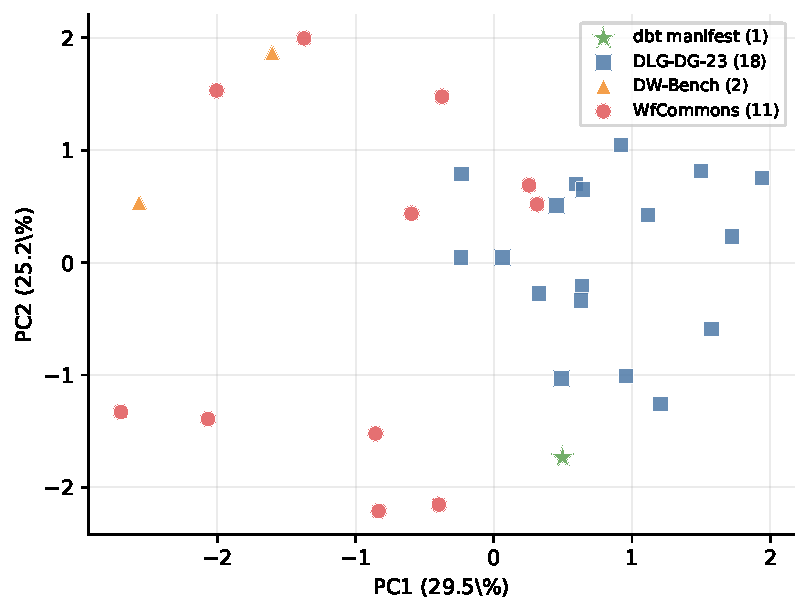
\includegraphics[width=0.78\linewidth]{figures/crossdataset_pca.pdf}
\caption{PCA of five standardized descriptors (D1 CSI, D2 max Gini,
  D3 norm.\ gap, D3 Fiedler bim., D4 cycle rank/N) for all 32 graphs
  (cycle rank/N is defined for every graph, so descriptor coverage is
  complete). PC1 (29.5\%) loads on high CSI /
  low norm.\ gap / low cycle rank; PC2 (25.2\%) on high Fiedler bim.\ /
  high Gini. Production lineage graphs (dbt, DLG-DG-23) occupy the
  high-CSI / low-gap region; WfCommons workflows span broader space.}
\label{fig:pca}
\end{figure}

These results show that the descriptors produce interpretable
variation across genuinely different pipeline architectures. The
convergence of dbt and DLG-DG-23 profiles, from different organizations
and technology stacks, suggests structural regularities in production
lineage graphs. Alternative explanations (domain differences, scale
effects) cannot be ruled out from a descriptive comparison alone, but
the consistency across 19 production lineage graphs from two source
ecosystems is informative.

\subsection{Experiment 6: Preliminary Cross-Organisation Comparison}

We attempt cross-organisation replication of the dbt D3 finding on two
public dbt projects (Cal-ITP, 631 models; Mattermost, 235 models).

\paragraph{Unit-of-analysis caveat.}
The replication faces an unavoidable construct-validity issue. In our
dbt case study, ``domain'' is an explicit metadata assignment
(\texttt{domain\_or\_team\_owner}) curated by the data team. Cal-ITP
and Mattermost do not consistently populate \texttt{meta.domain} or
\texttt{meta.owner} on most models; we therefore partition by two-level
folder path (e.g., \texttt{staging/gtfs}, \texttt{mart/payments}). Folder
structure in dbt projects often reflects pipeline-layer organisation
rather than business-domain assignment. The Cal-ITP and Mattermost
``domains'' are therefore not the same construct as the dbt case-study
domains. We report Experiment~6 as preliminary cross-organisation
exploration, not validated cross-organisation replication.

\begin{table}[htb]
\centering
\caption{D3 algebraic connectivity vs.\ documentation rate across three
  organisations. The dbt case uses metadata-assigned domains;
  Cal-ITP and Mattermost use folder-derived domains.}
\label{tab:crossorg}
\begin{tabular}{lllrrl}
\toprule
Organisation & Domain unit & $n$ & $\rho$ & perm.\ $p$ & 95\% CI \\
\midrule
dbt (this study) & metadata-assigned & 18 & $-0.708$ & 0.002 & $[-0.92, -0.27]$ \\
Cal-ITP & folder-derived & 26 & $+0.023$ & 0.911 & $[-0.42, +0.44]$ \\
Mattermost & folder-derived & 6 & $+0.812$ & 0.070 & $[+0.00, +1.00]$ \\
\bottomrule
\end{tabular}
\end{table}

Cal-ITP (26 analyzable domains, the largest external sample) shows no
association between any D1--D4 descriptor and documentation coverage
(all $p > 0.11$). The bootstrap 95\% confidence interval for D3 vs.\
doc\_rate spans zero. Mattermost ($n = 6$) shows a positive marginal
association ($\rho = +0.81$, $p = 0.070$), but the bootstrap CI is
$[+0.00, +1.00]$, because the sample size is too small for the bootstrap to
constrain the lower bound away from zero, so the directional reversal
relative to dbt is suggestive but not statistically supported.

Two readings are equally consistent with the data. Either (a) the original
dbt finding is organisation-specific and does not generalise (the
between-layer architecture interpretation from Experiment~2e); or (b)
the folder-derived domain construct in Cal-ITP and Mattermost is too
different from the metadata-assigned dbt domains to constitute a
proper replication attempt. We cannot distinguish these without
curated domain metadata from a third organisation. The honest
conclusion is that the dbt finding has not been replicated and will
not be replicable from public dbt projects alone at the graph-aggregate
level. Experiment 7 below pursues a different cross-organisation test
that succeeds at node granularity.

\subsection{Experiment 7: Core Data Asset Prediction on DLG-DG-23}

We extracted the expert-annotated core-asset labels from Table 5 of
\citet{chen2024dlgdg} and computed node-level topological features on
the six annotated graphs. Of 267 candidate Data Tables across the six
graphs, 36 are labeled core (class prevalence 13.5\%; per-graph
prevalence ranges from 8.2\% in DLG11 to 28.6\% in DLG9).

\paragraph{Per-feature univariate AUC.}
On the pooled set of 267 Data Tables, the strongest univariate
predictors of core status are reverse-PageRank on DATA\_FLOW (AUC =
0.778), PageRank on DATA\_FLOW (0.733), the corresponding ancestor count
(0.704), and in/out-degree (0.679 / 0.664). Local clustering on the
undirected projection is uninformative (constant zero on Data Table
nodes whose neighbourhoods are bipartite-to-fields).

\paragraph{Leave-one-graph-out cross-validation.}
We train logistic regression and random forest classifiers on five
graphs and predict core-asset status on the held-out sixth, repeating
for each graph (Table~\ref{tab:dlg_prediction}). The logistic-regression
standardizer is fitted on the five training graphs inside each fold;
the random forest receives unscaled features.

\begin{table}[htb]
\centering
\small
\caption{Leave-one-graph-out core-asset prediction on DLG-DG-23
  (Table 5 of \citep{chen2024dlgdg}). Bootstrap 95\% CIs from 2,000
  resamples per fold. LR = logistic regression, RF = random forest,
  both class-balanced.}
\label{tab:dlg_prediction}
\begin{tabular}{lrrrrr}
\toprule
Held-out graph & $n_{\text{test}}$ & core & LR AUC & 95\% CI & RF AUC \\
\midrule
DLG1 & 15 & 3 & 0.722 & $[0.385, 1.000]$ & 0.722 \\
DLG2 & 21 & 5 & 0.950 & $[0.822, 1.000]$ & 0.975 \\
DLG9 & 28 & 8 & 0.812 & $[0.612, 0.963]$ & 0.794 \\
DLG11 & 73 & 6 & 0.950 & $[0.885, 1.000]$ & 0.960 \\
DLG13 & 105 & 11 & 0.954 & $[0.875, 1.000]$ & 0.921 \\
DLG15 & 25 & 3 & 1.000 & $[1.000, 1.000]$ & 0.939 \\
\midrule
Mean $\pm$ std & & & $0.898 \pm 0.098$ & & $0.885 \pm 0.094$ \\
Random baseline & & & $0.546 \pm 0.127$ & & \\
Out-degree only & & & $0.576 \pm 0.155$ & & \\
\bottomrule
\multicolumn{6}{l}{\small One-sample $t$-test vs $\text{AUC}=0.5$ gives
LR $t=9.12$, $p=0.0003$ and RF $t=9.18$, $p=0.0003$.}
\end{tabular}
\end{table}

The multi-feature classifiers substantially outperform both the random
baseline and any single-feature baseline. The smallest held-out graph
(DLG1, 15 Data Tables) has wide bootstrap CIs reflecting limited
test-set power; the four medium and larger graphs (DLG2, DLG11, DLG13,
DLG15) achieve AUC $\geq 0.95$. Figure~\ref{fig:dlg_prediction} shows
the per-fold ROC curves and random-forest feature importance.

\begin{figure}[htb]
\centering
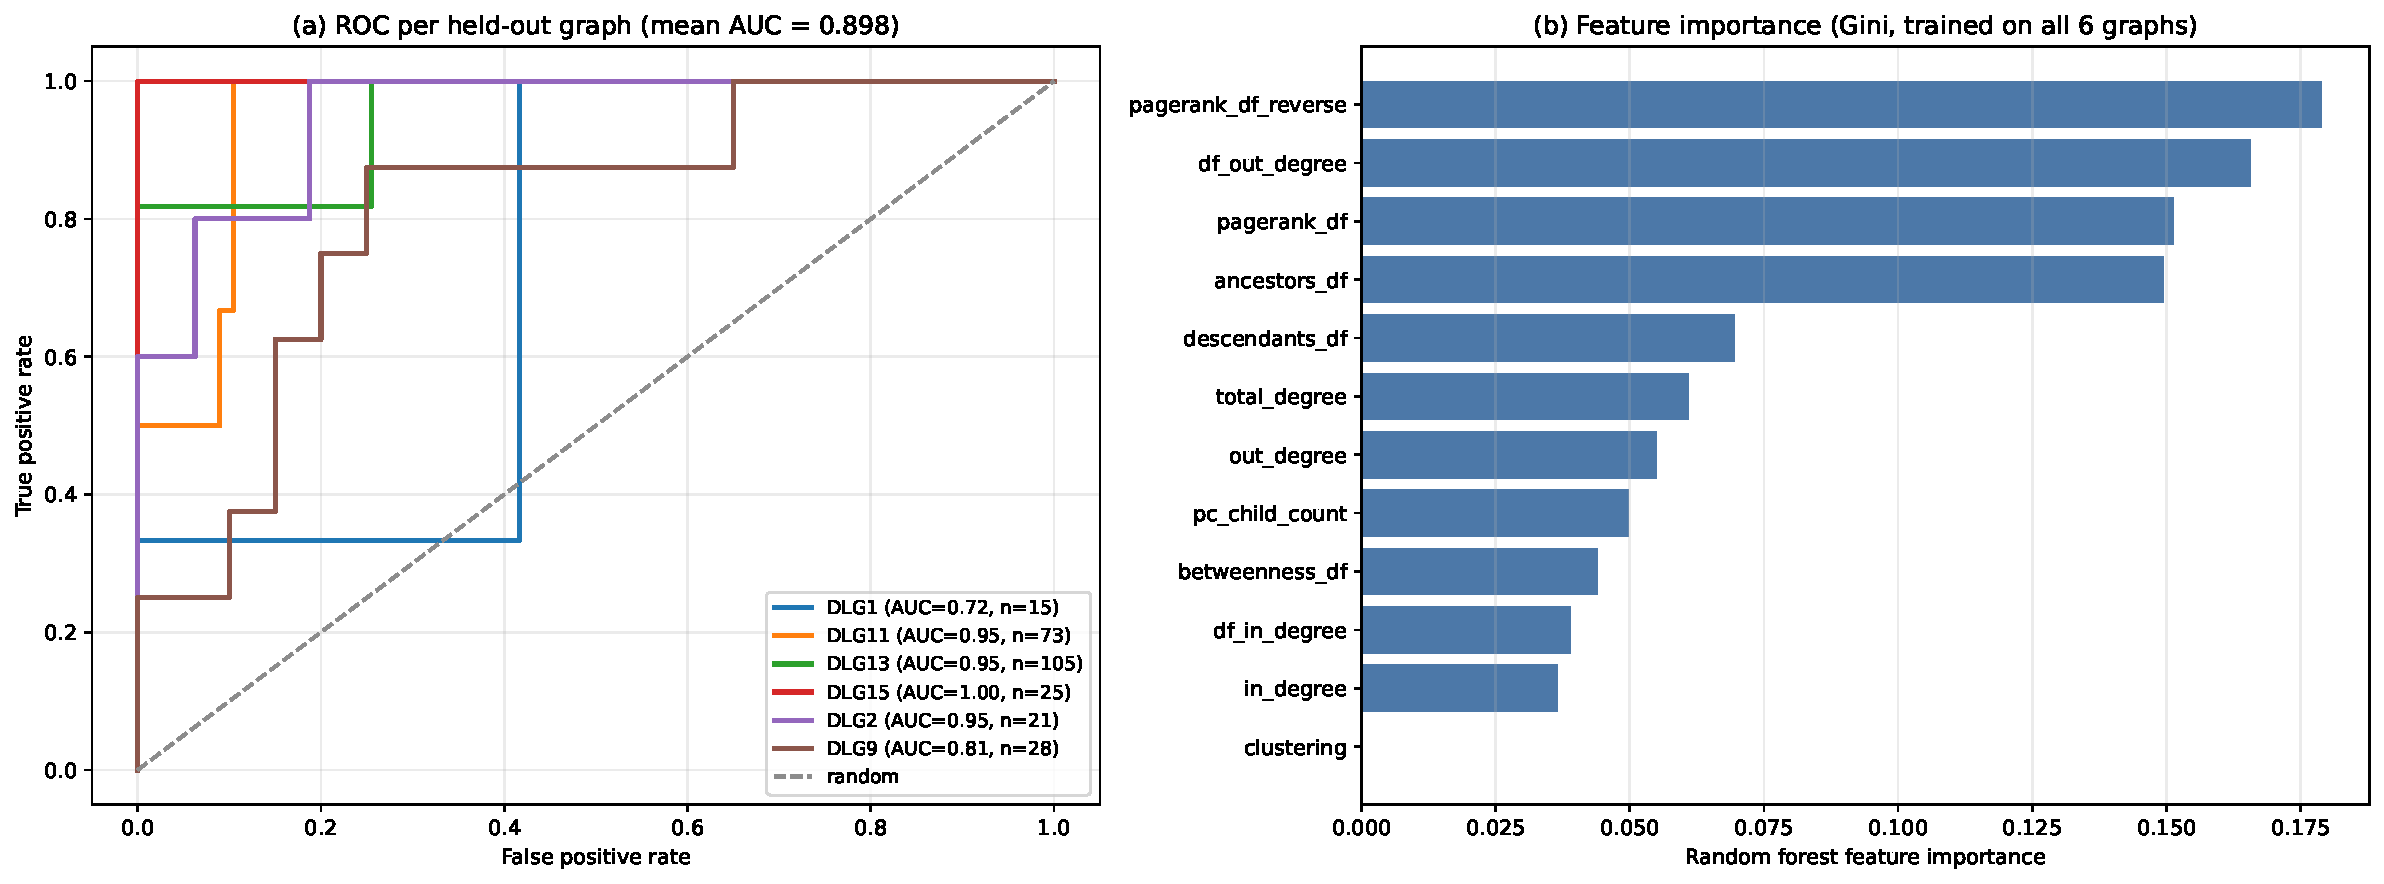
\includegraphics[width=0.97\linewidth]{figures/dlg_core_asset_prediction.pdf}
\caption{(a) ROC curve per held-out graph (LR classifier). (b) Random
  forest feature importance (Gini, trained on all 6 graphs).
  DATA\_FLOW reverse-PageRank and DATA\_FLOW out-degree are the most
  informative features.}
\label{fig:dlg_prediction}
\end{figure}

\paragraph{Shared-ID sensitivity.}
Three core-asset IDs appear in two graphs each. DLG9 and DLG15 share one;
DLG11 and DLG13 share two. To verify the result is not an artifact of
identical assets appearing in train and test sets with similar
topological features, we re-ran the leave-one-graph-out evaluation
with these IDs removed from each test set. The mean LR AUC drops only
from $0.898$ to $0.891$ (Table~\ref{tab:dlg_sensitivity}), confirming
that the predictive signal is not a leakage artifact.

\begin{table}[htb]
\centering
\small
\caption{Sensitivity analysis. Leave-one-graph-out LR AUC with the
  three shared core-asset IDs excluded from each test set.}
\label{tab:dlg_sensitivity}
\begin{tabular}{lrr}
\toprule
Held-out graph & IDs removed & LR AUC (excl. shared) \\
\midrule
DLG1 & 0 & 0.722 \\
DLG2 & 0 & 0.950 \\
DLG9 & 1 & 0.807 \\
DLG11 & 2 & 0.925 \\
DLG13 & 2 & 0.943 \\
DLG15 & 1 & 1.000 \\
\midrule
Mean & & $0.891 \pm 0.096$ \\
\bottomrule
\end{tabular}
\end{table}

\paragraph{Interpretation.}
Two structural properties dominate, DATA\_FLOW reverse-PageRank
(importance 0.179) and DATA\_FLOW out-degree (0.166). A high
reverse-PageRank value indicates that random walks starting from
downstream nodes are biased toward the node in question; substantively,
the table is an upstream source for many downstream consumers. High
DATA\_FLOW out-degree is the local version of the same property, since
the table is directly read by many downstream jobs. Both align with
the expert annotation rationale described in \citet{chen2024dlgdg},
that ``T1 is a core data asset because it serves as a base table for
generating new tables.''

The result is a reproduction of the node-centrality finding of
\citet{chen2023centrality} on the same DLG-DG-23 corpus, not a new
governance result. The two dominant predictors are centrality measures
(DATA\_FLOW reverse-PageRank and out-degree). Because the feature set
does not contain node-level versions of D1--D4, this experiment cannot
estimate their incremental value. We report the AUC to confirm that
lineage structure encodes node-importance signal captured by simple
centrality, and to delineate a boundary condition.
Node-level expert labels yield a tractable supervised learning problem
that centrality already solves, whereas domain-level continuous metadata
aggregated across heterogeneous layers does not yield a within-layer
governance signal at all (Experiments 2--6).

\subsection{Experiment 4: Predictive Comparison}

\begin{table}[htb]
\centering
\caption{Prediction performance (5-fold cross-validation, 120 samples).}
\label{tab:exp4}
\begin{tabular}{llrr}
\toprule
Task & Feature set & Baselines & Multi-scale \\
\midrule
Classification (AUC) & Logistic & 1.000 & 1.000 \\
Classification (AUC) & Random Forest & 1.000 & 1.000 \\
Regression $R^2$ (MTTD) & Ridge & 0.246 & 0.277 \\
Regression $R^2$ (MTTD) & Random Forest & 0.175 & 0.307 \\
\bottomrule
\end{tabular}
\end{table}

Standard 5-fold cross-validation achieves ceiling AUC = 1.0 for all
feature sets, confirming that synthetic governance variation produces
structurally separable graphs but providing no discriminative evidence
between feature sets at this evaluation. Leave-scale-out cross-validation
(training on three scales, testing on the held-out scale) gives a more
stringent test of generalisation across graph sizes. Under this scheme,
baselines achieve AUC = 1.000 across all four held-out folds; multi-scale
descriptors achieve AUC = 0.935 $\pm$ 0.113, dropping to 0.74 when
medium-scale graphs are held out. Baselines, which include diameter and
degree statistics that scale predictably with graph size, generalise
better across scales than the multi-scale features in this controlled
experiment. The MTTD regression result ($R^2 = 0.307$ for multi-scale vs.\
$0.175$ for baselines) should be read in that light, since the gain may
not hold on graph sizes outside the training distribution.

\textbf{D1 seed robustness on synthetic graphs.}
Running 25 Louvain seeds per condition reveals that D1 differentiation
survives seed noise only at large scale. Separation between well and
poor governance as a multiple of seed standard deviation (SNR) runs
tiny $= -0.5\times$ (well CSI lower than poor), small $= 0.9\times$,
medium $= 0.8\times$, large $= 2.8\times$. At tiny through medium
scales, Louvain seed variance is comparable to or larger than the
governance-level separation, making single-seed D1 results at those
scales unreliable. The large-scale D1 result (mean separation 0.307,
SNR $2.8\times$) is the only scale where the differentiation clearly exceeds
optimizer noise.

\section{Discussion}

\subsection{Which Descriptors Survive Scrutiny}

The convergent evidence from synthetic experiments, real-data
correlations, partial correlations, and null models identifies which
descriptors capture governance-relevant structure and which do not.

D1 CSI differentiates synthetic governance levels after FDR correction
($d = 3.9$ at large scale) and the null model confirms it captures
structure beyond degree sequences ($z = +3.7$). Seed robustness
analysis qualifies this. At large scale the separation between well
and poor governance exceeds seed variance by 2.8×, but at tiny through
medium scales the seed variance is comparable to the governance
separation, making those results unreliable. The large-scale synthetic
result and the null model finding are the most defensible evidence for
D1. Real-data correlation with governance metadata is not directly
testable because most domain subgraphs lack internal edges for
meaningful community detection.

D3 algebraic connectivity showed the strongest initial real-data
correlation ($\rho = -0.71$ vs.\ documentation, FDR $p = 0.043$), but
subset robustness analysis and layer-stratified permutation reveal this
is a between-layer architectural artifact, with D3 = 0 for source
domains, D3 = 1.0 for silver domains, and an intermediate value for
gold/mart. The association
does not survive restriction to domains with internal edges (Subset B,
$n = 6$, FDR $p = 0.19$). The null model agrees. D3 algebraic
connectivity is degree-sequence-determined ($z = -0.42$) and captures no
hidden structural signal. D3 characterizes layer architecture reliably,
but cannot distinguish governance levels within layers.

D3 Fiedler bimodality is the most striking null model result ($z = -23.8$).
The real graph has dramatically lower bimodality than degree-matched
random graphs, suggesting that the real graph's Fiedler vector reflects
genuine organizational structure (a smooth gradient across pipeline
layers) rather than the sharp random bipartitions that emerge from
rewiring.

D4 H1 features differentiate governance levels in synthetic experiments
and capture structure beyond degree sequences ($z = -2.95$), while
cycle rank does not ($z = +0.88$). This is the setting where persistent
homology adds value over the simpler baseline. When testing whether
structure goes beyond what degree sequences determine, cycle rank
trivially passes (it is nearly preserved by rewiring), while H1
features provide a meaningful test.

D3 normalized spectral gap fails both the partial correlation test (sign
reversal, $p = 0.49$) and the null model ($z = -0.38$). Its apparent
real-data correlation was confounded by domain size.

\subsection{What the Layer Confound Means for Structural Governance
Measurement}

Section~\ref{sec:degeneracy} establishes the mechanism. Here we take the
consequence, which reaches past this estate and past this descriptor.

We did not simply pick a bad descriptor. The problem is that the
partition which governance metadata attaches to, the domain, sits nested
inside the partition which architecture imposes, the layer. Domain
membership and layer membership are close to collinear in a medallion
estate, because a domain of raw sources and a domain of staging models
are different kinds of object rather than two samples of one kind. Any
descriptor computed on domain subgraphs will therefore separate layers
before it separates anything else, and any governance attribute that
also varies by layer, as documentation and test coverage both do, will
correlate with that separation. D3 is where the effect is easiest to
see, since $\lambda_2$ is pinned to closed-form values on edgeless
graphs and on stars, but D3 is not the only descriptor exposed to it.

That reframes what a structural governance measurement would have to
demonstrate. Reporting a correlation is not enough, and neither is
controlling for domain size, which we also did and which leaves the D3
association standing (partial $\rho = -0.55$, $p = 0.021$) because size
is not the confound. The requirement is a design in which governance
quality varies within an architectural stratum, so that the stratified
test has something to detect. Our estate supplies no such stratum. Its
five staging domains have documentation rate zero without exception and
its mart layer has one member.

D3 does identify layer boundaries reliably, and that is a real if modest
structural finding. It is simply not the finding the hypothesis needed.

\subsection{Limitations}

\textbf{Rank-degenerate D3 in the dbt sample.} D3 algebraic connectivity
takes only three distinct values across the 18 analyzable dbt domains,
so the $\rho = -0.71$ correlation is a three-tier ordering test and
cannot resolve within-tier variation. The descriptor is not at fault.
The values are pinned by how production dbt domains decompose into
edgeless source clusters, staging stars, and a handful of reticulated
mart domains. We want to be careful about the remedy, because the
obvious one does not work. Collecting a larger estate of the same
architecture yields more observations at $\lambda_2 \in \{0, 1\}$ rather
than more distinct values, so sample size is not the binding
constraint. What would relax it is an estate whose domains cut across
layers rather than sitting inside them, or per-asset governance metadata
that permits a unit of analysis other than the domain. Both are
availability problems rather than statistical ones.

\textbf{Effect size at detection threshold.} Power analysis under the
observed rank degeneracy shows minimum detectable $|\rho|$ at 80\% power
is $0.7$--$0.8$ for $n = 18$. The observed $|\rho| = 0.71$ for D3 vs.\
doc\_rate is at this threshold. The dataset cannot distinguish a true
correlation of $0.71$ from a true correlation of $0.85$.

\textbf{Cross-organisation construct mismatch.} The Cal-ITP and Mattermost
domains are folder-derived, while the dbt case study domains are metadata-
assigned. Folder structure in dbt projects often reflects pipeline-layer
organisation rather than business-domain assignment. The non-replication
in Experiment 6 therefore confounds (i) actual non-replication of the
governance--topology relationship with (ii) construct mismatch in the
unit of analysis. We cannot separate these without curated cross-
organisation metadata.

\textbf{D3 Fiedler bimodality null-model result is partly tautological.}
The $z = -23.8$ result reflects gross structural differences between
sparse layered DAGs and their degree-matched random rewirings (which tend
to be more bipartite-like). It does not isolate a subtle governance-
relevant property of the real graph.

\textbf{Generator circularity in synthetic experiment.} The generator's
\textit{well/baseline/poor} knobs control structural features (cross-layer
edge density, hub centrality) that overlap with what D1--D4 measure.
Experiment 1 should be read as a software-correctness / pipeline
validation step, not as external validation. The leave-scale-out CV
result (baselines AUC $= 1.000$ vs.\ multi-scale AUC $= 0.935 \pm 0.113$)
confirms multi-scale features do not generalise across scales better
than simple baselines in this controlled synthetic setting.

\textbf{D4 cycle rank equivalence on real data.} In both synthetic and
real-data settings, cycle rank $\beta_1 = M - N + C$ captures the same
governance correlation as H1 persistent features ($\rho = +1.000$ between
the two across domains). D4's added value over the simpler baseline is
restricted to null-model testing. For practical applications, cycle rank
may be sufficient and is vastly cheaper to compute.

\textbf{Missing metadata.} The production dbt catalog contains no
steward or owner metadata, reducing the governance score to a
two-component measure (tests + documentation). Organisations with
richer metadata would enable testing D1's hypothesised association
with ownership structure.

\textbf{Causal direction.} Correlations between descriptors and
governance metadata could reflect either direction, governance practices
producing cleaner structure, or cleaner structure making governance
easier. We measure association, not causation.

\subsection{Future Work: What Would Make the Question Answerable}
\label{sec:futurework}

The limitations above are not addressable from publicly available dbt
projects, and they are only partly addressable by collecting more data
of any kind. The binding requirement is a design in which the descriptor
is free to vary inside an architectural stratum. We set out what such a
study needs, in order of how hard each item is to obtain.

\begin{itemize}
  \item \textbf{Within-layer governance variation, first and without
        substitute.} The study needs domains where governance practice
        differs while architecture does not, for instance several mart
        domains in one organisation, some well tested and some not. Our
        estate has one mart and five staging domains whose documentation
        rate is uniformly zero, so there is no stratum in which a
        stratified test could detect anything. No amount of additional
        data with the same layer structure repairs this.

  \item \textbf{Curated domain-level metadata.} Explicit
        \texttt{meta.domain} or \texttt{meta.owner} assignments declared
        by data engineering teams rather than inferred from folder
        structure. Without it the unit-of-analysis problem from
        Experiment 6 recurs, and folder paths reintroduce exactly the
        layer confound the design is trying to escape.

  \item \textbf{Three to five organisations} willing to share lineage
        manifests and per-asset or per-domain governance metadata, under
        an NDA arrangement that preserves anonymisation while permitting
        topology--metadata analysis.

  \item \textbf{Enough analyzable domains to have power once the first
        item holds.} Twenty to thirty domains with $N \geq 5$ is a
        reasonable target, but the ordering matters. Sample size buys
        power only after within-layer variation exists, and buys nothing
        before that.

  \item \textbf{Versioned manifests over time}, six to twelve months of
        weekly snapshots, to support temporal change-detection studies
        that would shift the contribution from cross-sectional
        correlation to longitudinal governance drift.
\end{itemize}

The DLG-DG-23 authors confirmed in correspondence that no additional
core-asset annotations are available, so that route has reached its
label ceiling. Remaining routes include the OpenMetadata and DataHub
user communities, where some organisations publish anonymised catalogue
exports, and direct enterprise partnerships under NDA.

A separate preregistered successor study moves to a per-change unit,
with exact before/after dbt manifests, post-merge repairs adjudicated within
a fixed 30-day window, and declared tests, contracts, ownership, and
freshness as potential moderators. Its ordinary change statistics are
compared with global graph deltas and a separately named change-centred
geometry family. This follows change-level quality-assurance design
\citep{kamei2013large} while retaining whole-graph change measures such
as DeltaCon as baselines \citep{koutra2016deltacon}. No outcome model has
been fitted. One deliberately selected repair-linked feasibility case is
excluded from confirmation, and the consecutive outcome cohort will be
frozen before labels are opened. The successor is not empirical support
for the present paper; it is the protocol implied by this paper's
negative result.

\subsection{Practical Implications}

If validated on additional datasets, these descriptors could support
three uses.

\begin{enumerate}
  \item \textbf{Structural monitoring.} Computing D1 and D3 Fiedler
        bimodality on each CI/CD push provides a structural signal
        without manual assessment. CSI degradation over time signals
        erosion of domain boundaries.
  \item \textbf{Targeted intervention.} D3 identifies structurally
        isolated components. D2 identifies nodes with outsized blast
        radius. These guide where to invest governance effort.
  \item \textbf{Complementary evidence.} The descriptors complement
        existing governance frameworks by providing structural measurement
        where traditional methods provide periodic assessment.
\end{enumerate}

\section{Conclusion}

Institutional theory implies that governance maturity should leave a
structural signature in the artifacts governance produces. We tested
that implication on data lineage graphs and it does not hold, at least
not in a form a topological descriptor can recover from a domain-level
partition.

The apparent evidence looked strong and was spurious. D3
algebraic connectivity correlates with documentation rate at $\rho =
-0.71$ across 18 curated-metadata domains, with a bootstrap interval
clear of zero. The descriptor takes three values across those eighteen
domains and is constant inside each architectural layer, so
layer-stratified permutation returns $p = 1.000$ with a null $\rho$
standard deviation of exactly zero. Twelve source domains are edgeless
and give $\lambda_2 = 0$. Five staging domains are stars and give
$\lambda_2 = 1$ by the closed form. One mart sits between them. The
correlation orders three layers, and it says nothing about governance
within any of them.

We stress the mechanism rather than the null because the mechanism
travels and the null on its own does not. The three values are what a
medallion build pattern produces, so the degeneracy should be expected
in any estate organized that way, and a larger sample of such estates
supplies more observations at the same three values. A preliminary
cross-organisation comparison on two public dbt projects did not
replicate the finding either, though construct mismatch between
metadata-assigned and folder-derived domains prevents a clean
conclusion about replicability there.

Separately, and independent of the governance question, the descriptors
place production data lineage graphs from one dbt instance and 18 Huawei
Cloud DLGs in a distinct region of descriptor space, marked by high
community stability and small normalised spectral gaps and separable
from scientific workflow topologies. That characterization reproduces
and needs no governance metadata, which is why it stands while the
governance claim does not.

\textbf{At node granularity, a centrality-based prediction reproduces a
published result.} Using the expert-annotated core-asset labels
published in \citep{chen2024dlgdg} for six Huawei Cloud lineage graphs,
node-level topological features (DATA\_FLOW PageRank, ancestor count,
out-degree) predict core-asset status under leave-one-graph-out
cross-validation at LR AUC $= 0.898 \pm 0.098$ (random baseline
$0.546$, $p = 0.0003$). The result is robust to excluding shared
core-asset IDs (AUC $= 0.891$). The predictive signal is carried by
ordinary node features led by PageRank and out-degree. D1--D4 are not
features in this model, so no descriptor-versus-centrality comparison is
available. The AUC therefore reproduces the node-centrality finding of
\citet{chen2023centrality} on the same corpus rather than extending it.
We report it as such, not as a positive governance finding for the
descriptors.

We offer four things and we would rather label each of them accurately
than generously. The first is the bounded negative result above, with
its mechanism named. The second is a structural characterization across
32 lineage graphs from four sources, which needs no governance metadata
and does not depend on the failed hypothesis. The third is the inference
protocol. We transferred most of it from experimental design and network
science, and one component is new, the rank-degeneracy diagnostic that
would have flagged this design before anyone computed the correlation.
The fourth is a node-level core-asset prediction at AUC 0.90 that
reproduces the centrality finding of \citet{chen2023centrality} on the
Huawei Cloud DLGs. We report it as a reproduction because that is what
it is.

The practical reading is unglamorous and we think it is correct.
Governance maturity is better measured through process and curated
metadata than through graph structure, which is what the frameworks and
the commercial tooling already do. Where structure does carry a signal
about which assets matter, simple centrality recovers it. The
descriptors are still computable from any lineage graph, whether a dbt
manifest, a catalog export or a code-derived dependency graph, and they
still need no access to the underlying data, so the comparative
characterization remains useful. The governance prediction does not. We
would rather say so plainly than leave the question open for the next
group to rediscover at the same cost.

\appendix

\section{Reproducibility}

All code, anonymized data, and experiment scripts are archived at
Zenodo\footnote{Version DOI \href{https://doi.org/10.5281/zenodo.20209148}{10.5281/zenodo.20209148} for v2.1.0. The concept DOI \href{https://doi.org/10.5281/zenodo.20099999}{10.5281/zenodo.20099999} always resolves to the latest version.}
and on GitHub.\footnote{\url{https://github.com/mhdk1602/multiscale-governance-descriptors}}
The repository includes the following.

\begin{itemize}
  \item \texttt{src/governance\_descriptors/} is the Python package implementing
        D1--D4 and statistical utilities (permutation Spearman,
        Benjamini--Hochberg FDR, partial Spearman correlation).
  \item \texttt{experiments/} holds the experiment scripts that reproduce
        all tables in this paper.
  \item \texttt{data/} holds the anonymized dbt lineage data (HMAC-SHA256
        hashed node identifiers, domain labels, governance metadata).
\end{itemize}

\noindent\textbf{Dependencies.} Python 3.11+, NetworkX 3.x, NumPy, SciPy, pandas,
GUDHI (for persistent homology), scikit-learn (for Experiment 4).

\noindent\textbf{Anonymization.} All node identifiers, domain names, and schema
names in the production dbt data were replaced with HMAC-SHA256 hashes
prior to export. No organizational identifiers, table names, or column
names are present in the released data.

\bibliographystyle{plainnat}
\bibliography{references}

\end{document}
